\documentclass[12pt]{report}
\usepackage[utf8]{inputenc}
\usepackage[utf8]{vietnam}
\usepackage{amsmath}
\usepackage{amsfonts}
\usepackage{amssymb}
\usepackage{graphicx}
\usepackage{caption}
\usepackage{booktabs}
\usepackage{hyperref}
\usepackage{tabu}
\usepackage{indentfirst}
\usepackage{array}
\setlength{\parindent}{2em}
\renewcommand{\baselinestretch}{1.5}
\usepackage{tikz}
\usetikzlibrary{calc}
\usetikzlibrary{decorations.pathmorphing}
\usepackage{subcaption}
\usepackage{verbatim} 
\usepackage{listings}
\usepackage{lmodern}  % for bold teletype font
\usepackage{xcolor}   % for \textcolor
\setcounter{secnumdepth}{3}
\definecolor{light-gray}{gray}{0.95}
\lstset{
  language=Python,
  backgroundcolor=\color{light-gray},
  basicstyle=\ttfamily,
  frame=single,
  breaklines=true,
  postbreak=\mbox{\textcolor{red}{$\hookrightarrow$}\space},
}


%\renewcommand{\familydefault}{\sfdefault}


%
%\title{LaTex Thesis Template}	%% title
%\author{Trương Ngọc Anh}			%% author's name

%
\newcommand{\argmax}{\arg\!\max}

\begin{document}
\begin{titlepage}
\begin{tikzpicture}[overlay,remember picture]
    \draw [line width=0.5mm,decorate,decoration={
        %,segment length=<length>,amplitude=<length>
        }]
        ($ (current page.north west) + (3cm,-3cm) $)
        rectangle
        ($ (current page.south east) + (-3cm,3cm) $);
\end{tikzpicture}
\begin{center}
	\textbf{ĐẠI HỌC QUỐC GIA TP.HỒ CHÍ MINH}\\
	TRƯỜNG ĐẠI HỌC BÁCH KHOA\\
	KHOA KHOA HỌC VÀ KỸ THUẬT MÁY TÍNH\\
	---------------o0o--------------- \\
	\vspace{5mm}
	
\includegraphics[scale=0.2]{charts/logo.png}
\end{center}
\vspace{5mm}

\begin{center}
	\textbf{\small HỆ QUẢN TRỊ CƠ SỞ DỮ LIỆU}\\
	\textbf{\large Document Store (MongoDB, CouchDB, SimpleDB} 
\end{center}



\vspace{5mm}

\textbf{Giảng viên hướng dẫn: } Thầy Trần Quang

\vspace{5mm}

\textbf{Sinh viên thực hiện:}\\

 \begin{tabular}{| c | c |} 
 \hline
\textbf{ Họ và tên }& \textbf{MSSV} \\ [0.5ex] 
 \hline
 Trương Ngọc Anh & 1410141 \\ 
 \hline
 Lê Nguyễn Minh Trí & 1414207 \\
 \hline
 Nguyễn Quốc Kim Hoàng & 141xxxx \\
 \hline
 Nguyễn Khánh Bình & 141xxxx \\
 \hline
\end{tabular}
\thispagestyle{empty}
\end{titlepage}


%
\begin{comment}

\end{comment}
%\maketitle
\tableofcontents

%

%
\listoffigures
\listoftables
%\mainmatter
%
\chapter{Giới thiệu NoSQL và MongoDB}
\section{Mở đầu}
Hiện nay khi nói đến cơ sở dữ liệu, có sự phân chia rõ ràng giữa 2 trường phái kĩ thuật cơ sở dữ liệu là SQL và NoSQL - hay còn gọi cách khác là Cơ sở dữ liệu Quan hệ và Cơ sở dữ liệu Phi Quan hệ. Trong các chương trình giảng dạy ở bậc đại học thì thường chú trọng vào nghiên cứu và tìm hiểu các nguyên lý, cấu tạo của cơ sở dữ liệu SQL mà không khai thác các cơ sở dữ liệu NoSQL. Do đó ở bài báo cáo này, chúng ta sẽ tập trung tìm hiểu và khai thác kiến thức về các cơ sở dữ liệu NoSQL mà đối tượng nghiên cứu cụ thể tiêu biểu là MongoDB.

\section{NoSQL - Non SQL}
Đầu tiên, ta sẽ giới thiệu về NoSQL. Bên cạnh đó nêu ra cách phân loại các cơ sở dữ liệu NoSQL và nêu ra các điểm khác nhau nổi bật giữa cơ sở dữ liệu NoSQL và cơ sở dữ liệu quan hệ truyền thống.
\subsection{Giới thiệu}
Tuy NoSQL đã xuất hiện từ thập niên 60 nhưng thời gian gần đây nó mới bắt đầu tìm được vị trí của mình. Như tên gọi của nó, NoSQL cung cấp cơ chế triển khai cơ sở dữ liệu không theo cấu trúc nhất định. SQL đã tận dụng tốt việc khai báo schema chặt chẽ để quản lý, lưu trữ dữ liệu một cách tối ưu và cung cấp cho người dùng phương tiện để truy cập, sử dụng cơ sở dữ liệu hiệu quả nhất, nhờ đó mà nó đã từng là lựa chọn hàng đầu cho việc triển khai cơ sở dữ liệu.

Trong thời đại hiện nay, với sự bùng nổ của các dịch vụ internet kéo theo sự bùng nổ dữ liệu người dùng phi cấu trúc. Chính sự chặt chẽ của cơ sở dữ liệu SQL đã gây khó khăn trong việc quản lý, lưu trữ các dữ liệu phi cấu trúc này do SQL chỉ hoạt động tốt trên dữ liệu có cấu trúc. Điều này đã tạo cơ hội cho NoSQL phát huy điểm mạnh của mình.
\subsection{Phân loại}
Cơ sở dữ liệu NoSQL sử dụng khai báo schema động để quản lý cơ sở dữ liệu theo nhiều cách khác nhau, dựa vào đó ta có thể phân chúng thành nhiều loại:
\begin{itemize}
\item \textbf{Key-value store} mô hình SQL đơn giản nhất, lưu trữ dữ liệu dưới dạng khóa và trị. Tiêu biểu: ArangoDB, Aerospike, Oracle NoSQL Database, Dynamo, Riak, Voldemort.
\item \textbf{Column store} lưu các bảng dữ liệu theo dạng cột như đơn vị lưu trữ nhỏ nhất thay vì theo hàng như truyền thống. Tiêu biểu: Amazon DynamoDB, Bigtable, Cassandra, Druid, HBase, Hypertable.
\item \textbf{Document store} với ý tưởng chính là việc định nghĩa "document", là đơn vị dữ liệu nhỏ nhất chứa dữ liệu của bản thân nó và có mang key để phục vụ việc truy xuất. Ngoài việc truy xuất theo khóa thì các Document-Database này còn cung cấp các API giúp truy xuất document dựa trên nội dung nó chứa. Tiêu biểu: \textbf{\textit{MongoDB}}, ArangoDB, BaseX, Clusterpoint, Couchbase, CouchDB, DocumentDB, IBM Domino, MarkLogic, Qizx, RethinkDB.
\item \textbf{Graph} thường được dùng cho dữ liệu mà quan hệ giữa các thực thể có thể được biểu diễn tốt bằng đồ thị. Tiêu biểu: Neo4J, Polyglot.
\end{itemize}
\section{So sánh SQL và NoSQL}
\subsection{Query phức tạp}
Nhờ vào cấu trúc chặt chẽ của mình nên SQL có khả năng thực hiện các câu query phức tạp một cách tối ưu nhất so với NoSQL.
\subsection{ACID}
Tuân thủ ACID giúp CSDL SQL bảo vệ tính toàn vẹn, đảm bảo tính hợp lý của transaction. Tuy nhiên CSDL NoSQL bỏ qua ACID để có thể trở nên linh động và tăng tốc độ xử lý.
\subsection{Dữ liệu lưu trữ}
SQL chỉ có thể lưu trữ có cấu trúc. NoSQL có thể lưu trữ dữ liệu có cấu trúc hoặc phi cấu trúc.
\subsection{Khả năng mở rộng}
SQL khả mở rộng độ sâu của CSDL trong khi NoSQL khả mở rộng chiều ngang, giúp cho CSDL có thể được phân tán ở nhiều server qua đó tăng hiệu suất truy xuất dữ liệu, phù hợp cho các CSDL lớn và thay đổi liên tục.
\subsection{Cấu trúc}
Trong khi SQL ràng buộc việc khai báo schema rõ ràng trước khi có thể thêm dữ liệu thì với NoSQL ta có thể tạo document mà không cần khai báo schema trước. Mỗi document có cấu trúc, schema khác nhau.
\newpage
\section{MongoDB} \label{sec:MongoDB}
Sau khi đã tìm hiểu về NoSQL nói chung ở phần trước thì phần này ta sẽ đi vào chi tiết cụ thể về một điển hình tiêu biểu của NoSQL là MongoDB. Ở phần \ref{ssec:MongoDB.1} ta sẽ giới thiệu sơ bộ về MongoDB bên cạnh các khái niệm về các đơn vị và cấu trúc cơ bản của một CSDL xây dựng bằng MongoDB. Sau đó ta sẽ liệt kê sơ bộ các loại dữ liệu trong phần \ref{ssec:MongoDB.2} và các lệnh cơ bản nhất trong phần \ref{ssec:MongoDB.3}.
\subsection{Giới thiệu} \label{ssec:MongoDB.1}
MongoDB là hệ CSDL NoSQL Document store mở. Mỗi record trong MongoDB là một \textbf{\textit{document}}, gồm có các cặp trường và trị, và mỗi bảng sẽ là \textbf{\textit{collection}}, tập hợp nhiều document, và \textbf{\textit{Database}} là tập hợp của nhiều collection. Do cấu trúc linh động nên bảng không có schema cố định mà schema của mỗi document sẽ tự do document quản lý và quyết định. Document của MongoDB có cấu trúc gần giống với các đối tượng JSON. Các giá trị có thể là document khác hoặc mảng hoặc mảng các document.
\subsection{Datatype} \label{ssec:MongoDB.2}
Ngoài việc hỗ trợ các datatype thông dụng trong các ngôn ngữ lập trình, MongoDB còn định nghĩa một số datatype khác nhau:
\begin{itemize}
\item \textbf{Date}
\item \textbf{ObjectId} là kiểu dữ liệu được MongoDB dùng mặc định để đánh Id cho các document trong collection
\item \textbf{Số} MongoDB mặc định lưu trữ các dữ liệu số dưới dạng double 64-bit. Bên cạnh đó còn cung cấm nhiều wrapper để đặc tả các số một cách cụ thể như:
\begin{itemize}
\item \textbf{NumberLong} 64-bit integer
\item \textbf{NumberInt} 32-bit integer
\item \textbf{NumberDecimal} 128-bit decimal-based floating-point numbers
\end{itemize}
\end{itemize}
\subsection{Các thao tác cơ bản trong MongoDB sử dụng mongo shell - CRUD} \label{ssec:MongoDB.3}
\subsubsection{Create}
\begin{itemize}
\item 
\begin{lstlisting} 
use DATABASE_NAME
\end{lstlisting}
sẽ truy cập database có tên \textit{DATABASE\_NAME} hoặc tạo nếu chưa tồn tại và truy cập database vừa tạo.
\item 
\begin{lstlisting}
db.createCollection(collection_name, options)
\end{lstlisting}
dùng để tạo một collection tên \textit{collection\_name} và có thể khai báo thêm một số option như capped, size, max - Giới hạn kích thước hay số lượng document tối đa của collection - hay autoIndexId - tự động index trường \_id của document.
\item
\begin{lstlisting}
db.collection_name.insert(document)

db.collection_name.insertOne(document)
\end{lstlisting}
thêm \textit{document} vào collection \textit{collection\_name}
\item
\begin{lstlisting}
db.collection_name.insertMany(documents)
\end{lstlisting}
thêm tất cả các document trong danh sách \textit{documents} vào collection \textit{collection\_name}
\end{itemize}
\subsubsection{Read}
\begin{itemize}
\item
\begin{lstlisting}
show dbs
\end{lstlisting}
xuất cái database hiện có.
\item
\begin{lstlisting}
show collections
\end{lstlisting}
xuất danh sách các collection trong database hiện tại.
\item
\begin{lstlisting}
db.collection_name.find()
\end{lstlisting}
xuất tất cả document trong collection \textit{collection\_name}.
\item
\begin{lstlisting}
db.collection_name.find(query)
\end{lstlisting}
xuất tất cả document trong collection \textit{collection\_name} thỏa điều kiện \textit{query}.
\end{itemize}
\subsubsection{Update}
\begin{itemize}
\item
\begin{lstlisting}
db.colletion_name.updateOne(query, action)
\end{lstlisting}
thực hiện update được mô tả trong \textit{action} trên document thỏa điều kiện \textit{query} trong \textit{collection\_name}. Nếu có nhiều hơn 1 document thỏa \textit{query} thì sẽ thực hiện \textit{action} trên document đầu tiền thỏa.
\item
\begin{lstlisting}
db.colletion_name.updateMany(query, action)
\end{lstlisting}
thực hiện update được mô tả trong \textit{action} trên tất cả document thỏa điều kiện \textit{query} trong \textit{collection\_name}.
\item
\begin{lstlisting}
db.colletion_name.replaceOne(query, document)
\end{lstlisting}
thay thế document thỏa \textit{query} trong \textit{collection\_name} bằng \textit{document}. Nếu có nhiều hơn 1 document thỏa \textit{query} trong collection thì thực hiện thay thế trên document đầu tiên thỏa.
\end{itemize}
\subsubsection{Delete}
\begin{itemize}
\item
\begin{lstlisting}
db.dropDatabase()
\end{lstlisting}
dùng để xóa database đang truy cập.
\item
\begin{lstlisting}
db.collection_name.drop()
\end{lstlisting}
dùng để drop collection có tên \textit{collection\_name}
\item
\begin{lstlisting}
db.colletion_name.deleteOne(query)
\end{lstlisting}
xóa một document thỏa \textit{query} trong \textit{collection\_name}. Nếu có nhiều hơn 1 document thỏa \textit{query} trong collection thì xóa document đầu tiên thỏa.
\item
\begin{lstlisting}
db.colletion_name.deleteMany(filter)
\end{lstlisting}
xóa tất cả document thỏa \textit{filter} trong \textit{collection\_name}.
\end{itemize}
\subsection{Câu Query}
Câu query đóng vai trò quan trọng trong việc tìm kiếm, truy xuất, cập nhật Database. MongoDB cung cấp bộ quy tắc để viết các câu query tiện lợi, nhất quán.
\subsubsection{Cơ bản nhất}
\begin{lstlisting}
{<field>:<value>, ...}
\end{lstlisting}
Câu query cơ bản nhất trong MongoDB chính là so sánh bằng. Câu query cấu tạo từ các cặp khóa-trị với biểu diễn mối quan hệ trường và giá trị của trường, câu query sẽ truy xuất tất cả các document có trường được định trong \textit{<field>} có giá trị \textit{<value>}. Do câu query có cấu tạo là tập hợp nhiều cặp khóa-trị nên có bản chất \textit{AND}. Ví dụ như:
\begin{lstlisting}
db.NhanVien.find({luong:2000, mspb: "P01"})
\end{lstlisting}
câu query trên sẽ giúp phép find truy xuất tất cả các Nhân viên có \textit{lương} là 2000 và \textit{mspb} là 
"P01". Phép find cùng câu query trên tương tự như câu query trong SQL:
\begin{lstlisting}
select * from NhanVien where luong=2000 and mspb="P01"
\end{lstlisting}

Bên cạnh đó, ở \textit{\textbf{<value>}} ta có thể thay giá trị cụ thể bằng các kết hợp toán tử so sánh, OR, AND,... để phức tạp hóa câu query nhằm phục vụ mục đích của mình.
\subsubsection{Các toán tử so sánh để chọn}
Dùng các toán tử để chọn từ dữ liệu các document có giá trị trường \textit{<field>} thỏa:
\begin{itemize}
\item \lstinline!$eq! bằng. cú pháp: \lstinline!<field> : {$eq: <value>}! \\* ví dụ như \lstinline!db.NhanVien.find({luong: {$eq: 2000}})! truy xuất tất cả nhân viên có lương 2000. Tuy nhiên câu query trên cũng tương đương bản rút gọn ta đã tìm hiểu qua ở phần trước \lstinline!db.NhanVien.find({luong:2000})!.
\item \lstinline!$ne! không bằng. cú pháp: \lstinline!<field> : {$ne: <value>}! \\* ví dụ như \lstinline!db.NhanVien.find({luong: {$ne: 2000}})! truy xuất tất cả nhân viên có lương khác 2000.
\item \lstinline!$gt! lớn hơn. cú pháp: \lstinline!<field> : {$gt: <value>}! \\* ví dụ như \lstinline!db.NhanVien.find({luong: {$gt: 2000}})! truy xuất tất cả nhân viên có lương lớn hơn 2000.
\item \lstinline!$gte! lớn hơn hoặc bằng. cú pháp: \lstinline!<field> : {$gte: <value>}! \\* ví dụ như \lstinline!db.NhanVien.find({luong: {$gte: 2000}})! truy xuất tất cả nhân viên có lương lớn hơn hoặc bằng 2000.
\item \lstinline!$lt! nhỏ hơn. cú pháp: \lstinline!<field> : {$lt: <value>}! \\* ví dụ như \lstinline!db.NhanVien.find({luong: {$lt: 2000}})! truy xuất tất cả nhân viên có lương nhỏ hơn 2000.
\item \lstinline!$lte! nhỏ hơn hoặc bằng. \\* ví dụ như \lstinline!db.NhanVien.find({luong: {$lte: 2000}})! truy xuất tất cả nhân viên có lương nhỏ hơn hoặc bằng 2000.
\item \lstinline!$in! giá trị trong danh sách các giá trị được định. cú pháp: \lstinline!<field> : {$in: [<value0>, <value1>, ..., <valueN>]}! \\* ví dụ như \lstinline!db.NhanVien.find({mspb: {$in: ["P01","P04"]}})! truy xuất tất cả nhân viên thuộc phòng ban có mã số	trong danh sách \lstinline!["P01","P04"]! được định. Tác vụ trên tương đương câu query trong SQL \lstinline!select * from NhanVien where mspb in ("P01","P04")!.
\item \lstinline!$nin! giá trị không nằm trong danh sách các giá trị đã được định. cú pháp: \lstinline!<field> : {$nin: [<value0>, <value1>, ..., <valueN>]}! \\* ví dụ như \lstinline!db.NhanVien.find({mspb: {$nin: ["P01","P04"]}})! truy xuất tất cả nhân viên không thuộc phòng ban có mã số	trong danh sách \lstinline!["P01","P04"]! được định.
\end{itemize}
\subsubsection{Các toán tử logic}
Ngoài các toán tử so sánh toán học, MongoDB còn cung cấp các toán tử logic như:
\begin{itemize}
\item \lstinline!$and! cú pháp: \lstinline!{$and: [ {<expression0>}, {<expression1>}, ... ,{<expressionN>} ] }! với \textit{expression} là các câu điều query khác. \\* ví dụ như \lstinline!db.NhanVien.find({$and: [{luong: 2000}, {mspb:"P01"}]})! truy xuất tất cả nhân viên có lương 2000 và thuộc phòng ban có mspb "P01". Tác vụ truy xuất trên tương đương với câu query SQL \lstinline!select * from NhanVien where luong=2000 and mspb="P01"! . Ta có thể thấy nó tương đương với câu query cơ bản \lstinline!db.NhanVien.find({luong:2000},{mspb:"P01"})!.
\item \lstinline!$or! cú pháp: \lstinline!{$or: [ {<expression0>}, {<expression1>}, ... ,{<expressionN>} ] }! \\* ví dụ như \lstinline!db.NhanVien.find({$or: [ {luong:2000}, {mspb:"P02"}]})! truy xuất tất cả nhân viên có lương 2000 hoặc thuộc phòng ban có mã số "P02".
\item \lstinline!$not! truy xuất các document không thỏa điều kiện được định hoặc \textbf{không có trường được định}. cú pháp: \lstinline!{<field> : {$not: {<expression>}}}! với \textit{<expression>} là các cụm query bằng sử dụng toán tử toán học. \\* ví dụ như: \lstinline!db.NhanVien.find({ngay_nghi: {$not: {$gt: 3}}})! truy xuất tất cả nhân viên có ngày nghỉ \textit{bé hơn hoặc bằng} 3 hoặc \textbf{không có trường ngay\_nghi}.
\item \lstinline!$nor! áp dụng phép toán tử logic \textbf{nor}. cú pháp: \lstinline!{$nor: [ {<expression0>}, {<expression1>}, ... ,{<expressionN>} ] }! \\* ví dụ như \lstinline!db.NhanVien.find({$nor: [ {luong: 2000}, {mspb: "P01"} ] })! truy xuất các nhân viên thỏa:
\begin{itemize}
\item \textit{lương} khác 2000 và \textit{mspb} khác "P01"
\item \textit{lương} khác 2000 và không có trường \textit{mspb}
\item không có trường \textit{lương} và \textit{mspb} khác "P01"
\item không có cả trường \textit{lương} và trường \textit{mspb}
\end{itemize}
\end{itemize}
\section{Kiến trúc lưu trữ của MongoDB} \label{sec:MongoDB.4}
Cuối cùng, ở phần này ta sẽ đi chi tiết vào kiến trúc của MongoDB. Ta sẽ giới thiệu sơ về 2 định dạng dữ liệu JSON ở \ref{ssec:MongoDB.4.1} và BSON ở \ref{ssec:MongoDB.4.2}. Sau đó ta sẽ đi vào cốt lõi của việc lưu trữ dữ liệu của MongoDB trong phần \ref{ssec:MongoDB.4.3}.
\subsection{JSON} \label{ssec:MongoDB.4.1}
\textbf{JSON} (viết tắt cho \textit{JavaScript Object Notation}) là một định dạng lưu trữ, trao đổi dữ liệu nhẹ, con người có thể dễ dàng đọc và ghi cho cả con người và máy. JSON là định dạng được lưu dưới dạng text và không phụ thuộc vào ngôn ngữ lập trình sử dụng tuy cách kí hiệu gần gũi với các ngôn ngữ họ C như C, C++, C\#, Java, Javascript, Perl, Python,...

JSON được xây dựng dựa trên 2 cấu trúc dữ liệu nền tảng là:
\begin{itemize}
\item \textit{Tập hợp các cặp key-value (khóa-trị)} được gọi là \textit{object} (đối tượng).
\item \textit{Danh sách các giá trị} hay còn được gọi là \textit{array} (mảng).
\end{itemize}
Các loại dữ liệu (trị) mà JSON có thể nhận dạng là:
\begin{itemize}
\item string
\item number
\item object
\item array
\item true
\item false
\item null
\end{itemize}
\subsection{BSON} \label{ssec:MongoDB.4.2}
MongoDB lưu trữ dữ liệu dưới một phương thức biểu diễn nhị phân gọi là BSON. \textbf{BSON} (BinaryJSON) là phương thức mã hóa nhị phân các document với định dạng tương tự JSON. BSON còn mở rộng các kiểu dữ liệu, thêm vào một số kiểu dữ liệu mà JSON chưa có như Date, BinData.

Các thuộc tính chính của BSON:
\begin{itemize}
\item \textbf{Nhẹ}. Các overhead được tối giảm hết mức có thể.
\item \textbf{Khả duyệt tuần tự}. BSON được thiết kế có khả năng cho phép duyệt tuần tự dữ liệu.
\item \textbf{Hiệu quả}. Mã hóa và giải mã file BSON có thể được thực hiện nhanh chóng nhờ vào sử dụng các kiểu dữ liệu của C.
\end{itemize}
Ví dụ về mã hóa BSON:
\begin{lstlisting}

 {"hello": "world"}
->	

  \x16\x00\x00\x00                   // total document size
  \x02                               // 0x02 = type String
  hello\x00                          // field name
  \x06\x00\x00\x00world\x00          // field value
  \x00                               // 0x00 = type EOO ('end of object')

 {"BSON": ["awesome", 5.05, 1986]}
->	
  \x31\x00\x00\x00
  \x04BSON\x00
  \x26\x00\x00\x00
  \x02\x30\x00\x08\x00\x00\x00awesome\x00
  \x01\x31\x00\x33\x33\x33\x33\x33\x33\x14\x40
  \x10\x32\x00\xc2\x07\x00\x00
  \x00
  \x00
\end{lstlisting}
\subsection{Storage Engine} \label{ssec:MongoDB.4.3}
\textbf{Storage Engine} chính là bộ phận giữ vai trò quản lý lưu trữ dữ liệu trên bộ nhớ chính cũng như trên đĩa. MongoDB cho phép người dùng chọn các storage engine khác nhau trong nhiều trường hợp khác nhau. Việc chọn storage engine phù hợp với mục đích sử dụng sẽ giúp cải thiện hiệu năng của hệ thống sử dụng cơ sở dữ liệu.
\subsubsection{WiredTiger}
\textbf{WiredTiger} là storage engine mặc định kể từ MongoDB 3.2 trở đi. WiredTiger xuất hiện và thể hiện được sự mạnh mẽ của mình, qua đó trở thành lựa chọn thông dụng trong việc xây dựng CSDL.

WiredTiger kiểm soát song song hóa ở tầng document (\textbf{Document-level Concurrency Control}) cho các tác vụ ghi. Việc này có nghĩa là nhiều user có thể ghi đồng thời nhiều document khác nhau trong cùng một collection một cách song song. Phần lớn các tác vụ đọc, ghi được WiredTiger kiểm soát bằng Optimistic concurrency control. Khi phát hiện xung đột giữa 2 tác vụ, một trong 2 sẽ phát lỗi ghi dữ liệu khiến MongoDB sẽ thử thực hiện lại tác vụ đó sau.

Bên cạnh đó WiredTiger còn sử dụng \textbf{MultiVersion Concurrency Control} (MVCC). Khi bắt đầu tác vụ, WiredTiger sẽ tạo một \textbf{snapshot} - bản sao dữ liệu của cơ sở dữ liệu - thể hiện một phần nhỏ cơ sở dữ liệu vào trong bộ nhớ chính. Khi ghi xuống đĩa, WiredTiger ghi tất cả dữ liệu trong snapshot xuống đĩa. Dữ liệu lúc này đã trở nên bền vững và được xem là một checkpoint. \textbf{Checkpoint} có nhiệm vụ đảm bảo tính nhất quán của các file dữ liệu của cơ sở dữ liệu. Từ phiên bản \textit{3.6} thì WiredTiger tạo checkpoint mỗi 60 giây. Trong khi đang ghi checkpoint mới thì checkpoint cũ hợp lệ sẽ vẫn được giữ nên nếu có trường hợp xảy ra lỗi khi đang ghi dữ liệu xuống đĩa thì ta vẫn có thể khôi phục lại đến checkpoint cũ. Checkpoint mới chỉ được xem là bền vững khi bảng metadata của WiredTiger được cập nhật đồng nhất để tham chiếu đến checkpoint mới, khi đó checkpoint cũ mới được xóa.

Tuy với WiredTiger ta có thể khôi phục đến checkpoint cuối cùng nhưng để khôi phục các thay đổi sau checkpoint đó thì ta cần sử dụng thêm ghi log. WiredTiger sử dụng \textit{write-ahead transaction log} - tức là các thay đổi tạo ra do các transaction được log ghi nhận chỉ được phép ghi xuống đĩa nếu log đó đã được ghi xuống đĩa.

Với WiredTiger, MongoDB hỗ trợ nén dữ liệu cho tất cả collection và index. Nén giữ liệu sử dụng thêm năng suất từ CPU đổi lại giúp giảm dung lượng sử dụng của cơ sở dữ liệu. Mặc định WiredTiger dùng thư viện \textit{snappy} để nén các block dữ liệu và file log. Bên cạnh đó ta có thể chọn không nén dữ liệu hoặc nén bằng thuật toán khác như \textit{zlib}.
\subsubsection{MMAPv1}
\textbf{MMAPv1} là storage engine cơ bản của MongoDB dựa trên memory mapped file với các ưu điểm về hoạt động tốt với các tác vụ insert, reads số lượng lớn và in-place update.

Để đảm bảo tính bền vững của cơ sở dữ liệu, MongoDB mặc định ghi log tất cả các thay đổi vào file log (journal) trên đĩa. MongoDB ghi log thường xuyên hơn là ghi dữ liệu xuống đĩa. Mặc định ghi dữ liệu xuống đĩa mỗi 60 giấy còn ghi log mỗi 100 mili giây. Chính việc ghi log giúp MongoDB khôi phục dữ liệu khi xảy ra sự cố.

Các record sẽ được cấp phát bộ nhớ liên tục trên đĩa, dùng để lưu trữ các document. Nếu document trở nên lớn hơn kích thước record đã được cấp phát thì record mới sẽ được cấp phát và document sẽ được dời sang record mới đồng thời cập nhất các tham chiếu index tới document đó.
\subsubsection{So sánh WiredTiger và MMAPv1}
\begin{itemize}
\item \textbf{Song song}

MMAPv1 sử dụng Collection-level Concurrency Control. Nếu một người dùng thực hiện tác vụ thay đổi một document thì cả collection của document đó sẽ bị lock và các người dùng khác sẽ không thể truy cập collection đó. Ở các phiên bản trước thì MMAPv1 dùng Database-level Concurrency Control.

Còn WiredTiger sử dụng Document-level, Optimistic Concurrency Control.
\item \textbf{Logging (Journal)}

MMAPv1 dùng tính năng này để khôi phục.

WiredTiger sử dụng các checkpoint để khôi phục dữ liệu, có thể dùng thêm logging để khôi phục các thay đổi chưa được tạo checkpoint.
\item \textbf{Nén dữ liệu}

MMAPv1 không nén dữ liệu trong khi WiredTiger có thể nén dữ liệu theo giải thuật snappy hay zlib.
\end{itemize}
\subsubsection{In-memory Storage Engine}
Như tên gọi, \textbf{In-memory Storage Engine} lưu trữ toàn bộ dữ liệu, dữ kiện thiết lập, index,... trên bộ nhớ chính. Vì thế giảm thiểu lượng lớn thời gian hao tổn do các tác vụ I/O trên đĩa. In-memory Storage Engine chỉ dành cho phiên bản \textit{MongoDB Enterprise}.

In-memory Storage Engine dùng Document-level Concurrency Control.

Do toàn bộ dữ liệu chỉ được lưu trữ trên bộ nhớ chính nên đổi lại năng suất, tốc độ cao thì CSDL không có tính bền vững.\newpage\cleardoublepage
\chapter{Thiết kế cơ sở dữ liệu với MongoDB}

\section{Index trong MongoDB}\cite{def}
\subsection{Index là gì?}
Trong cơ sở dữ liệu, ta đã biết Index(chỉ mục) là một file cấu trúc lưu trữ trên ổ cứng tương ứng với một table hoặc một view nào đó trong cơ sở dữ liệu nhằm mục đích cải thiện tốc độ truy xuất dữ liệu từ table hoặc view đó.\\
Ở mục này, chúng ta sẽ tìm hiểu cách đánh index cũng như các loại index có trong MongoDB.
\subsection{Các loại index}

\subsubsection{Compound index (Chỉ mục hỗn hợp các khóa)}
Đây là chỉ mục được đánh trên nhiều trường khác nhau trong database. Loại index nay hữu ích khi chúng ta thực hiện câu truy vấn trên đòi hỏi nhiều trường trên dữ liệu. Ví dụ câu lệnh sau đây giúp tạo chỉ mục hỗn hợp các khóa trên MongoDB.\\
\begin{figure}[h!]
		\centering
		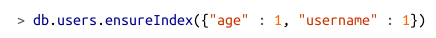
\includegraphics[scale=0.8]{charts/cpindex1.png}
		\caption{Câu lệnh tạo index hỗn hợp các khóa}
		\label{fig:cpindex}
\end{figure}
Trong câu lệnh trên, ta giả sử có một thư mục data có nhiều trường trong đó có trường username và age. Câu lệnh trên sẽ tạo ra chỉ mục đánh trên hai trường username và age đó. Số ứng với mỗi khóa trong câu lệnh chỉ mục trên thể hiện hướng của dữ liệu trên trường đó được sắp xếp như thế nào, với 1 là tăng dần, -1 là giảm dần. Trong ví dụ này thì age và username đều được đánh chỉ mục tăng dần.\\
Nếu ta có một tập dữ liệu gồm mà mỗi document trong dữ liệu đó bao gồm username có các giá trị như \textit{user01, user02, user03...} và age bao gồm các giá trị nguyên như \textit{1, 2, 3, 4...}. Thì chỉ mục sẽ có hình dạng như thế này
\pagebreak 
\begin{figure}[h!]
		\centering
		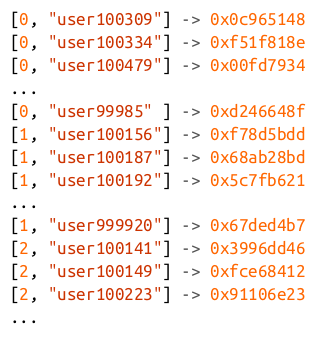
\includegraphics[scale=0.5]{charts/result.png}
		\caption{Kết quả}
		\label{fig:result}
\end{figure}
Mỗi index entry sẽ chứa lần lượt các giá trị của các trường là age ứng với giá trị nguyên và trường username ứng với các username \textit{user1, user2,...}. Và trong file index ấy do câu lệnh tạo index phía trên với trường age đứng trước tiên nên các entry được xếp tăng dần theo trường age và tiếp đến là tăng dần theo trường username có nghĩa là trước tiên chúng sắp xếp tăng dần theo trường age là số tuổi, tiếp đó với các user có cùng số tuổi thì sẽ sắp xếp tăng dần theo username. Bên cạnh đó, mỗi entry còn trỏ đến địa chỉ \textit{(được biểu diễn bằng chuỗi Hex)} của document được lưu trên đĩa.

\subsubsection{Unique index (Chỉ mục duy nhất)}
Với các hệ cơ sở dữ liệu như oracle, mySQL,... ta có primary index là dạng index đối với các trường có các giá trị không trùng nhau(unique). Với mongoDB, ta có Unique index hay còn gọi là chỉ mục duy nhất, các trường được đánh index này không được trùng nhau. Trong collection của mongoDB, trường "id" sẽ được tự động đánh là unique index.
\begin{itemize}
	\item \textbf{Compound unique index: }đây là sự kết hợp chỉ mục duy nhất với chỉ mục hỗn hợp các khóa. Cụ thể là, nếu có hai trường như name và address được đánh compound unique index thì một trong hai trường có thể có giá trị trùng nhau giữa các document nhưng không có document nào mà giống nhau ở cả hai trường đã được đánh index.
	\item \textbf{Các giá trị null: }trong quá trình insert dữ liệu, nếu một trường không có giá trị nào khi insert thi mongoDB sẽ mặc định giá trị đó là null. Nhưng nếu trường nói trên được đánh chỉ mục duy nhất thì nếu có thêm một trường bị gán giá trị null thì sẽ báo lỗi insert do trùng giá trị null.
\end{itemize}
\subsubsection{Sparse index (Chỉ mục thưa)}
Ở phần trên đề cập đến việc những trường được đánh chỉ mục duy nhất nhưng lại xuất hiện giá trị null. Trong những trường hợp có một trường nào đó trong collection mà có hoặc không cần insert giá trị nhưng bắt buộc trường đó là unique thì khi đó ta tạo chỉ mục duy nhất kết hợp với option sparse(thưa).\\
Ví dụ dưới đây là câu lệnh thực hiện việc tạo ra chỉ mục duy nhất trên trường email mà trường này không nhất thiết phải có giá trị. Các giá trị cấu hình cho unique và sparse lần lượt là "1" và "true":
\begin{figure}[h!]
		\centering
		
\includegraphics[scale=0.5]{charts/sparse.png}
		\caption{tạo chỉ mục duy nhất kết hợp với option sparse}
		\label{fig:spindex}
\end{figure}

\section{Aggregation}\cite{def1}
Sau khi data đã được lưu và thực hiện tạo index cần thiết trên mongoDB, trong công việc chúng ta có thể cần thực hiện nhiều tác vụ như phân tích theo nhiều cách khác nhau. Chính vì vậy mà mongoDB đã cung cấp một số công cụ để thực hiện các việc đó.\\
\subsection{Aggregation framework}
Aggragation có thể hiểu là sự tập hợp. Các Aggregation operation xử lý các bản dữ liệu và trả về kết quả đã được tính toán thành công. Các phép toán Aggregation nhóm các giá trị từ nhiều Document lại với nhau sau đó thực hiện nhiều phép toán đa dạng khác để trả về một kết quả duy nhất. Nói tới đây chúng ta liên tưởng tới phép toán count() và GROUPBY trong các hệ cơ sở dữ liệu SQL, các phép toán này tương ứng với Aggregation trong mongoDB.\\
Với Aggregation, mongoDB có hỗ trợ việc sử dụng thực hiện pipeline, có nghĩa là cho phép tạo ra một hoạt động hay tiến trình trên một số input và sử dụng output đó trở thành input cho các lệnh tiếp theo. Có một tập hợp các trạng thái có thể có, mỗi giai đoạn trên lấy một tập các document và tạo kết quả mà kết quả này được sử dụng cho các giai đoạn tiếp theo.
\textbf{Các giai đoạn trong Aggregation:}
\begin{itemize}
	\item \$match: công dụng như câu lệnh where trong các hệ cơ sở dữ liệu thông thường. Nó là hoạt động lọc giúp giảm số lượng document.
	\item \$project: giúp chọn một số trường cụ thể trong collection.
	\item \$group: thực hiện tập hợp lại các bản dữ liệu như phần đầu mục đã trình bày.
	\item \$sort: sắp xếp các document
	\item \$limit: giới hạn số document
	\item \$skip: Bỏ qua hay nhảy qua số document đã cung cấp.
	\item \$unwind: chia một document thành nhiều document. Tạo ra một số lượng document cho các giai đoạn khác nhau.
\end{itemize}
\pagebreak
\subsection{MapReduce}
MapReduce là hệ xử lý dữ liệu để tổng hợp (cô đọng) một khối lượng dữ liệu lớn thành các kết quả tổng thể có ích. Tuy nhiên đây là một công việc tốn kém về thời và không nên sử dụng cho việc phân tích dữ liệu real-time(thơi gian thực). Dưới đây là minh họa cho công việc MapReduce.\\
\begin{figure}[h!]
		\centering
		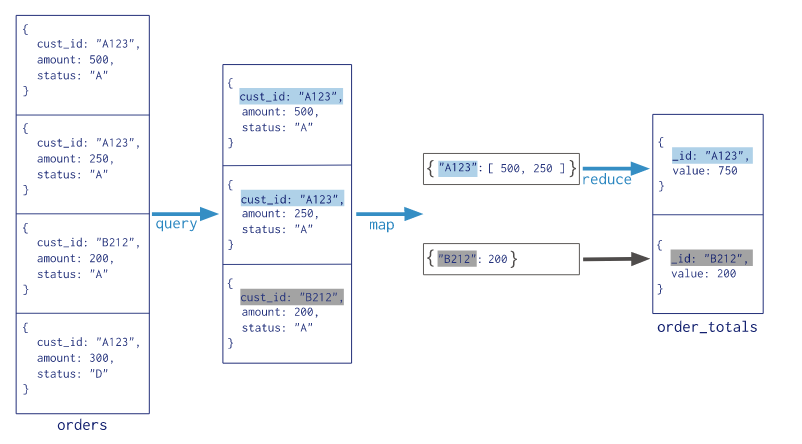
\includegraphics[scale=0.5]{charts/mapreduce.png}
		\caption{MapReduce}\cite{def3}
		\label{fig:mapreduce}
\end{figure}
Như hình trên, MapReduce gồm 2 bước chính. Thứ nhất là bước map, bước này mục đích là gộp các giá trị của các document khác nhau nhưng có chung một Key, như hình trên gom các giá trị của các document có key là "A123" lại với nhau và tương tự với key "B212". Bước tiếp theo là Reduce có nghĩa là rút gọn và gom hay tổng các giá trị cùng một Key được map ở bước trên (Hình minh họa)


\section{Các đặc điểm khi thiết kế cơ sở dữ liệu với MongoDB}\cite{def2}
\subsection{Normalization và Denormalization(Chuẩn hóa và không chuẩn hóa}
\textbf{Normalization (chuẩn hóa).} Khi thiết kế một hệ cơ sở dữ liệu nhằm mục đích trình bày cấu trúc của dữ liệu, chuẩn hóa là một trong những yếu tố quan trọng nhất. Chuẩn hóa trong store document là việc chia nhỏ dữ liệu ra nhiều collection và việc tham chiếu lẫn nhau giữa các collection. Vì thế nên có thể nhiều document có thể tham chiếu tới một mẫu dữ liệu nào trong một collection. Do tính chất đó mà khi cần thêm vào hay thay đổi dữ liệu được trỏ tới thì chỉ cần thay đổi tại một nơi. Tuy nhiên trong mongoDB thì việc query để thu thập các document sẽ là một câu query mà chứa nhiều câu query nhỏ.\\
\textbf{Denormalization (Không chuẩn hóa).} Ngược lại với chuẩn hóa, không chuẩn hóa không chia nhỏ dữ liệu hay nhiều document thao khảo thới một collection nào đó mà là việc nhúng một mẫu document này trong hoàn toàn một document khác, điều nay khiến cho việc update hay insert diễn ra khác khó khăn và phức tạp. Tuy nhiên không chuẩn hóa lại giúp việc đọc hay truy xuất dữ liệu nhanh hơn.\\
Do các yếu tố đặc điểm của store document trên mà việc lựa chọn chuẩn hóa hay không chuẩn hóa dữ liệu là một quyết định khó khăn. Trong những trường hợp cụ thể mà người thiết kế schema dưới dạng store document cần tính toán sao cho chuẩn hóa và không chuẩn hóa có lợi nhất.
\subsection{Ví dụ về trình bày dữ liệu trong store document}
Dưới đây la một ví dụ chuẩn hóa dữ liệu.
\begin{figure}[h!]
		\centering
		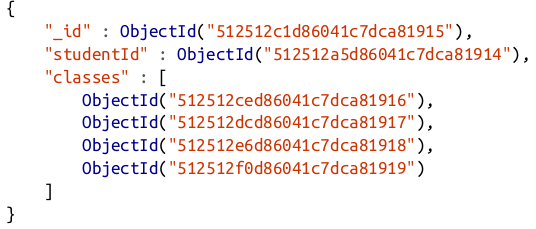
\includegraphics[scale=0.5]{charts/nor1.png}
		\caption{data representation 1}
		\label{fig:datare}
\end{figure}
Có thể thấy đây là một document chứa thông tin một sinh viên, trường id là biểu diễn id cho document đó ta bỏ qua, trường \textbf{studentId} chứa giá trị là một chuỗi Hex và có trường \textbf{classes} là một mảng chứa các đối tượng lưu những mã Hex khác nhau. Giờ đến với hình minh họa tiếp theo.
\begin{figure}[h!]
		\centering
		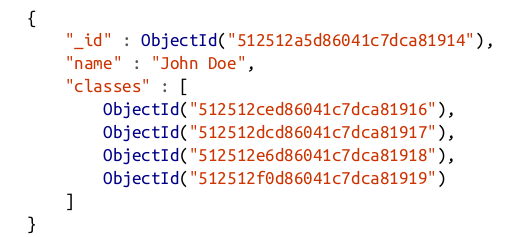
\includegraphics[scale=0.5]{charts/nor2.png}
		\caption{data representation 2}
		\label{fig:datare2}
\end{figure}
Với document này, ta chú ý đến trường \textbf{\_id} giá trị Hex của trường này trùng với giá trị Hex trong trường \textbf{studentId} của hình \ref{fig:datare}. Có nghĩa rằng trường \textbf{studentId} thao khảo đến document \ref{fig:datare2} la một sinh viên nào đó tên "John Doe". Cứ theo ý nghĩa trên, ta có thể nhận thấy rằng giá giá trị Hex trong mảng \textbf{classes} sẽ tham khảo đến một document nào đó mang thông tin lớp học mà có \textbf{\_id} trùng với giá trị mà nó mang.\\
Nếu muốn biểu diễn dữ liệu để tối ưu việt đọc truy xuất mà không quan tâm đến chi phí update thì dữ liệu thường được biểu diễn mọi thông tin class hay tên họ của sinh viên sẽ được lưu thẳng trực tiếp vào một document như sau mà không cần sử dụng việc tham khảo như trên. Đây là không chuẩn hóa đã được trình bày lý thuyết ở mục trên.
\begin{figure}[h!]
		\centering
		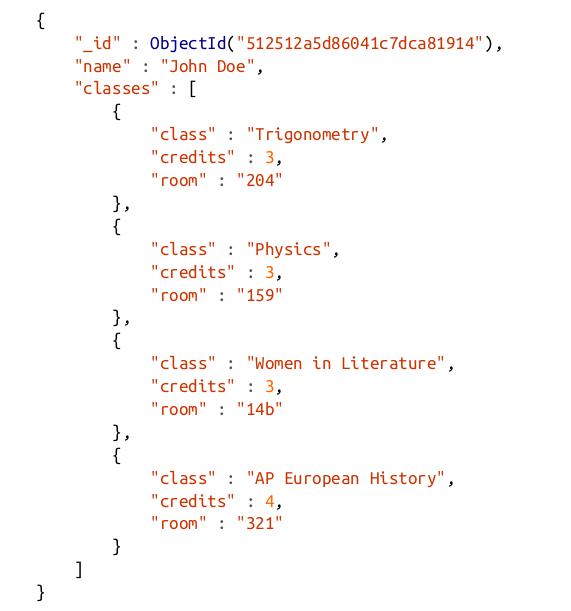
\includegraphics[scale=0.5]{charts/denor.png}
		\caption{dữ liệu không chuẩn hóa}
		\label{fig:datare3}
\end{figure}
\newpage\cleardoublepage
\chapter{Sharding} 
Sharding là một phương pháp phân phối dữ liệu trên nhiều máy. MongoDB sử dụng sharding để hỗ trợ triển khai với các tập dữ liệu rất lớn và các hoạt động thông lượng cao.

Các hệ thống cơ sở dữ liệu với các tập dữ liệu lớn hoặc các ứng dụng thông lượng cao có thể thách thức khả năng của một máy chủ đơn lẻ. Ví dụ, tỷ lệ truy vấn cao có thể làm cạn kiệt dung lượng CPU của máy chủ. Các kích thước bộ làm việc lớn hơn RAM của hệ thống làm tăng dung lượng I / O của ổ đĩa.

Có hai phương pháp để giải quyết sự tăng trưởng hệ thống: mở rộng theo chiều dọc và chiều ngang.

Chia tỷ lệ theo chiều dọc liên quan đến việc tăng dung lượng của một máy chủ đơn lẻ, chẳng hạn như sử dụng CPU mạnh hơn, tăng thêm RAM hoặc tăng dung lượng bộ nhớ. Các hạn chế trong công nghệ có sẵn có thể hạn chế một máy duy nhất không đủ mạnh cho một khối lượng công việc đã cho. Ngoài ra, các nhà cung cấp dựa trên đám mây có trần cứng dựa trên các cấu hình phần cứng có sẵn. Kết quả là, có tối đa thực tế cho việc mở rộng theo chiều dọc.

Chia tỷ lệ theo chiều ngang liên quan đến việc chia bộ dữ liệu hệ thống và tải trên nhiều máy chủ, thêm máy chủ bổ sung để tăng dung lượng theo yêu cầu. Mặc dù tốc độ hoặc dung lượng tổng thể của một máy đơn có thể không cao, mỗi máy sẽ xử lý một tập hợp con của khối lượng công việc tổng thể, có khả năng mang lại hiệu quả tốt hơn so với một máy chủ dung lượng cao tốc độ cao duy nhất. Việc mở rộng khả năng triển khai chỉ yêu cầu thêm các máy chủ bổ sung nếu cần, có thể thấp hơn tổng chi phí so với phần cứng cao cấp cho một máy. Cân  sự phức tạp trong cơ sở hạ tầng và bảo trì cho việc triển khai.

MongoDB hỗ trợ mở rộng theo chiều ngang thông qua sharding.

\section{Sharded Cluster}
Một cụm MongoDB shard bao gồm các thành phần sau:

\begin{itemize}
\item shard: Mỗi shard chứa một tập con của dữ liệu được shard. Mỗi shard có thể được triển khai như một bộ bản sao.
\item mongos: Các mongos hoạt động như một bộ định tuyến truy vấn, cung cấp một giao diện giữa các ứng dụng máy khách và cụm shard.
\item máy chủ cấu hình: Máy chủ cấu hình lưu trữ cài đặt siêu dữ liệu và cấu hình cho cụm. Theo MongoDB 3.4, các máy chủ cấu hình phải được triển khai như một bộ bản sao (CSRS).
\end{itemize}
Đồ họa sau đây mô tả sự tương tác của các thành phần trong một cụm shard:

\begin{figure}[h!]
\centering
\captionsetup{justification=centering,margin=1cm}
  	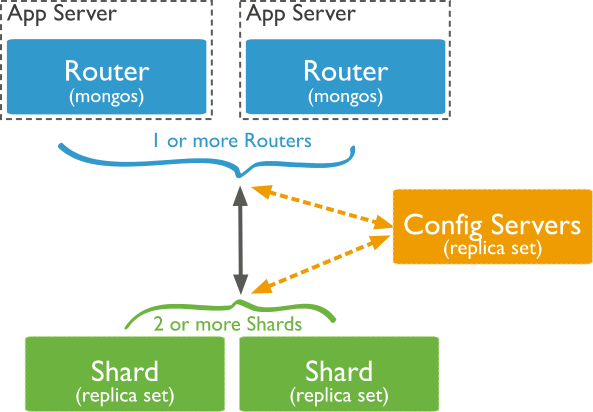
\includegraphics[scale=0.5]{charts/sharded-cluster-production-architecture.png}
  \caption{Sơ đồ của một cụm mẫu shard cho mục đích sản xuất. Chứa chính xác 3 máy chủ cấu hình, 2 hoặc nhiều bộ định tuyến truy vấn $`mongos`$ và ít nhất 2 mảnh. Các mảnh là bộ bản sao.}
  \end{figure}

MongoDB phân chia dữ liệu ở cấp thu thập, phân phối dữ liệu thu thập trên các shard trong cụm.

\section{Shard Keys}
Để phân phối các tài liệu trong một bộ sưu tập, MongoDB phân vùng bộ sưu tập bằng cách sử dụng khóa shard. Khóa shard bao gồm một trường hoặc trường bất biến tồn tại trong mọi tài liệu trong bộ sưu tập đích.

Bạn chọn khoá shard khi sharding một bộ sưu tập. Không thể thay đổi khóa shard sau khi sharding. Bộ sưu tập được phân loại có thể chỉ có một khóa shard. 

Để shard một bộ sưu tập không trống, bộ sưu tập phải có chỉ mục bắt đầu bằng khóa shard. Đối với các bộ sưu tập rỗng, MongoDB tạo chỉ mục nếu bộ sưu tập không có chỉ mục thích hợp cho khóa shard đã chỉ định. 

Sự lựa chọn của shard key ảnh hưởng đến hiệu suất, hiệu quả và khả năng mở rộng của một cluster bị phân mảnh. Một cụm với phần cứng và cơ sở hạ tầng tốt nhất có thể bị tắc nghẽn bởi sự lựa chọn của khóa shard. Việc lựa chọn mã khóa và chỉ số sao lưu của nó cũng có thể ảnh hưởng đến chiến lược tích trữ mà cụm của bạn có thể sử dụng.

\section{Chunk}
Các phân vùng MongoDB phân chia dữ liệu thành các đoạn. Mỗi đoạn có một cận trên và dưới dựa trên khoá shard.

MongoDB di chuyển các đoạn trên các mảnh trong cluster bị phân mảnh bằng cách sử dụng cân bằng cluster bị phân mảnh. Các cân bằng cố gắng để đạt được một sự cân bằng thậm chí của khối trên tất cả các mảnh trong cụm.

\section{Ưu điểm của Sharding}
\paragraph{Đọc / ghi}
MongoDB phân phối khối lượng công việc đọc và ghi trên các shard trong cụm shard, cho phép mỗi shard xử lý một tập con của các phép toán cụm. Cả hai khối lượng công việc đọc và ghi có thể được thu nhỏ theo chiều ngang trên cụm bằng cách thêm nhiều shard hơn.

Đối với các truy vấn bao gồm khóa shard hoặc tiền tố của khóa shard phức hợp, mongos có thể nhắm mục tiêu truy vấn tại shard cụ thể hoặc tập hợp các shard. Các hoạt động được nhắm mục tiêu này thường hiệu quả hơn là phát sóng tới mọi shard trong cụm.

\paragraph{Khả năng lưu trữ}
Sharding phân phối dữ liệu trên các shard trong cụm, cho phép mỗi shard chứa một tập hợp con của tổng số dữ liệu cụm. Khi tập dữ liệu phát triển, các shard bổ sung sẽ tăng dung lượng lưu trữ của cụm.

\paragraph{Tính sẵn sàng cao}
Một cụm shard có thể tiếp tục thực hiện một phần hoạt động đọc / ghi ngay cả khi một hoặc nhiều shard không có sẵn. Mặc dù tập hợp con dữ liệu trên các shard không có sẵn không thể truy cập được trong thời gian ngừng hoạt động, nhưng việc đọc hoặc viết trực tiếp tại các shard có sẵn vẫn có thể thành công.

Trong môi trường sản phẩm, shard cá nhân nên được triển khai dưới dạng bản sao, cung cấp khả năng dự phòng và tính khả dụng cao hơn.

\section{Cân nhắc trước khi Sharding}
Yêu cầu cơ sở hạ tầng cụm phức tạp và yêu cầu phức tạp đòi hỏi phải lập kế hoạch, thực hiện và bảo trì cẩn thận.

Cân nhắc cẩn thận trong việc chọn khóa shard là cần thiết để đảm bảo hiệu suất và hiệu quả của cụm. Bạn không thể thay đổi khóa shard sau khi sharding, cũng không thể unshard một bộ sưu tập sharded. Xem Chọn một khóa shard.

Sharding có một số yêu cầu và hạn chế hoạt động nhất định. Xem các hạn chế hoạt động trong các cụm đã shard để biết thêm thông tin.

Nếu các truy vấn không bao gồm khóa shard hoặc tiền tố của khóa shard hợp chất, mongos thực hiện một hoạt động phát sóng, truy vấn tất cả các shard trong cụm bị phân mảnh. Các truy vấn phân tán / thu thập này có thể là các hoạt động chạy dài.

\section{Sharded and Non-Sharded Collections}
Một cơ sở dữ liệu có thể có một hỗn hợp các bộ sưu tập bị phân mảnh và không bị trầy xước. Các bộ sưu tập được phân chia được shard và phân phối trên các shard trong cụm. Bộ sưu tập chưa được lưu trữ được lưu trữ trên shard chính. Mỗi cơ sở dữ liệu có shard chính của riêng nó.

\begin{figure}[h!]
\centering
\captionsetup{justification=centering,margin=1cm}
  	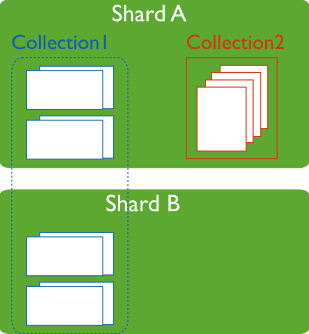
\includegraphics[scale=0.5]{charts/sharded-cluster-primary-shard.png}
  \caption{Sơ đồ shard chính. Phân đoạn chính chứa các bộ sưu tập không bị shard cũng như các khối tài liệu từ các bộ sưu tập được phân loại. Shard A là shard chính.}
  \end{figure}

\section{Kết nối với một cụm được shard}
Bạn phải kết nối với bộ định tuyến mongos để tương tác với bất kỳ bộ sưu tập nào trong cụm được shard. Điều này bao gồm các bộ sưu tập bị phân tán và không bị trói buộc. Khách hàng không bao giờ nên kết nối với một mảnh duy nhất để thực hiện các hoạt động đọc hoặc ghi.

\begin{figure}[h!]
\centering
\captionsetup{justification=centering,margin=1cm}
  	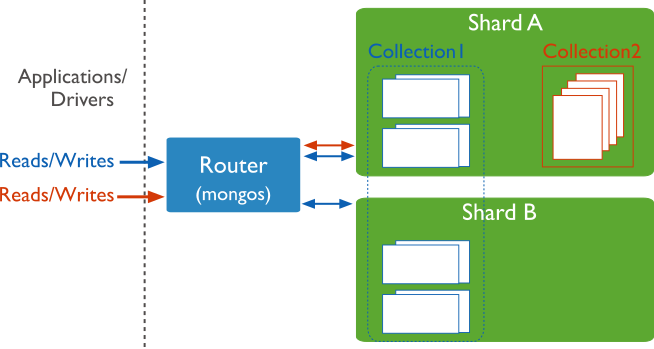
\includegraphics[scale=0.5]{charts/sharded-cluster-mixed.png}
  \caption{Sơ đồ các ứng dụng / trình điều khiển đưa ra các truy vấn tới mongos cho bộ sưu tập không bị quản lý cũng như bộ sưu tập được phân loại. Máy chủ cấu hình không được hiển thị. Bạn có thể kết nối với một mongos giống như cách bạn kết nối với một Mongod, chẳng hạn như thông qua trình bao mongo hoặc trình điều khiển MongoDB.}
  \end{figure}

Bạn có thể kết nối với một mongos giống như cách bạn kết nối với một Mongod, chẳng hạn như thông qua trình bao mongo hoặc trình điều khiển MongoDB.

\section{Sharding Strategy}
MongoDB hỗ trợ hai chiến lược sharding để phân phối dữ liệu trên các cụm bị phân mảnh.

\paragraph{Hashed Sharding}
Hashed Sharding liên quan đến việc tính toán giá trị băm của giá trị của trường khóa. Mỗi đoạn sau đó được gán một phạm vi dựa trên các giá trị khóa shard băm.

\begin{figure}[h!]
\centering
\captionsetup{justification=centering,margin=1cm}
  	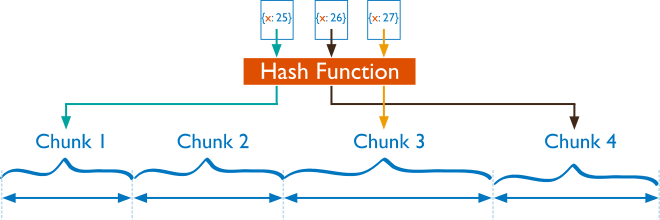
\includegraphics[scale=0.5]{charts/sharding-hash-based.png}
  \caption{Sơ đồ shard dựa trên băm.}
  \end{figure}

Mặc dù một loạt các khóa shard có thể là “đóng”, nhưng các giá trị băm của chúng không thể ở cùng một đoạn. Phân phối dữ liệu dựa trên các giá trị băm tạo điều kiện phân phối dữ liệu thậm chí nhiều hơn, đặc biệt là trong các tập dữ liệu trong đó khóa phân tử thay đổi một cách đơn điệu.

Tuy nhiên, phân phối băm có nghĩa là các truy vấn dựa trên phạm vi trên khóa shard ít có khả năng nhắm mục tiêu một shard đơn lẻ, dẫn đến nhiều hoạt động phát rộng hơn theo cụm

\paragraph{Ranged Sharding}
Sự phân rã có phạm vi liên quan đến việc chia dữ liệu thành các phạm vi dựa trên các giá trị khóa shard. Mỗi đoạn sau đó được gán một phạm vi dựa trên các giá trị khóa shard.

\begin{figure}[h!]
\centering
\captionsetup{justification=centering,margin=1cm}
  	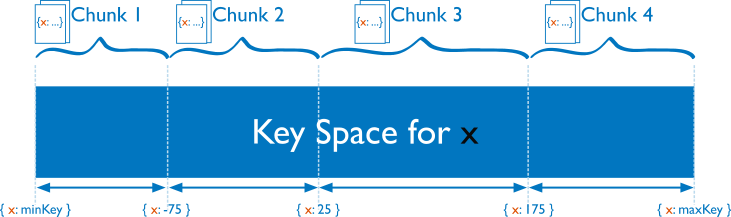
\includegraphics[scale=0.5]{charts/sharding-range-based.png}
  \caption{Sơ đồ không gian giá trị khóa shard được chia thành các phạm vi hoặc khối nhỏ hơn.}
  \end{figure}

Một loạt các khóa shard có giá trị “đóng” có nhiều khả năng cư trú trên cùng một đoạn. Điều này cho phép các hoạt động được nhắm mục tiêu như một mongos có thể định tuyến các hoạt động đến chỉ các mảnh có chứa dữ liệu cần thiết.

Hiệu quả của sharding dao động phụ thuộc vào phím shard được chọn. Các khóa shard kém được xem là có thể dẫn đến phân phối dữ liệu không đồng đều, có thể phủ nhận một số lợi ích của việc tích trữ hoặc có thể gây ra tắc nghẽn hiệu suất.

\section{Zones in Sharded Clusters}
Trong các cụm shard, bạn có thể tạo các vùng dữ liệu được phân loại dựa trên khóa shard. Bạn có thể kết hợp từng vùng với một hoặc nhiều mảnh trong cụm. Phân đoạn có thể kết hợp với bất kỳ số vùng nào. Trong một cụm cân bằng, MongoDB di chuyển các khối được bao phủ bởi một vùng chỉ cho các mảnh vỡ liên kết với vùng đó.

Mỗi vùng bao gồm một hoặc nhiều dải giá trị khóa shard. Mỗi phạm vi một vùng bao gồm luôn luôn bao gồm ranh giới thấp hơn của nó và độc quyền của ranh giới trên của nó.

\begin{figure}[h!]
\centering
\captionsetup{justification=centering,margin=1cm}
  	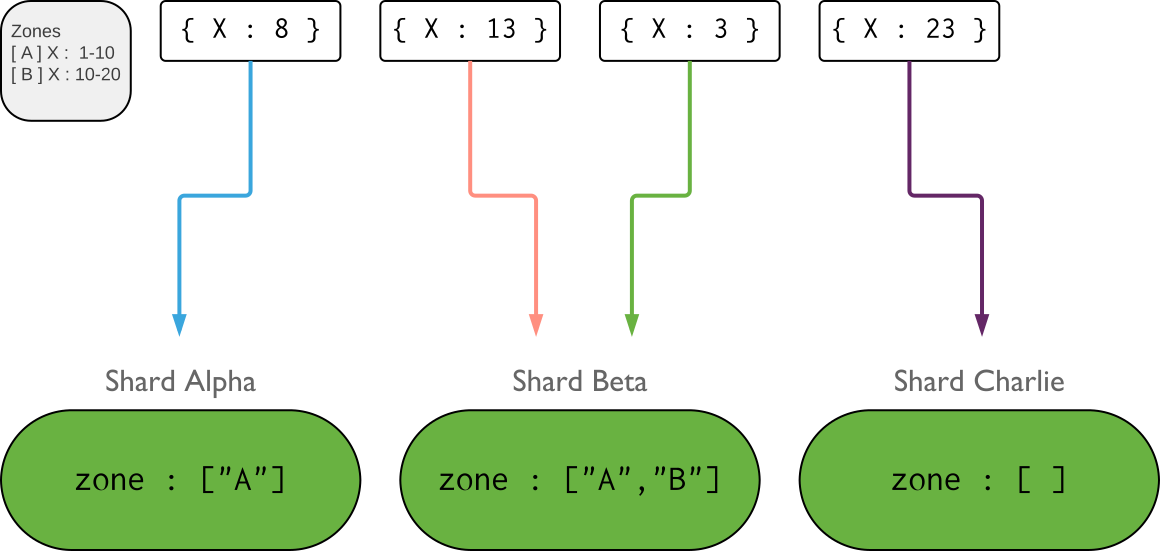
\includegraphics[scale=0.5]{charts/sharded-cluster-zones.png}
  \caption{Sơ đồ phân bố dữ liệu dựa trên các vùng trong một cụm shard}
  \end{figure}

Bạn phải sử dụng các trường có trong khóa shard khi xác định phạm vi mới cho vùng cần bao gồm. Nếu sử dụng khóa shard hợp chất, phạm vi phải bao gồm tiền tố của khóa shard. 

Khi chọn một khóa shard, hãy xem xét cẩn thận khả năng sử dụng sharding khu vực trong tương lai, vì bạn không thể thay đổi khóa shard sau khi sharding bộ sưu tập.

Phổ biến nhất, các khu vực phục vụ để cải thiện địa phương của dữ liệu cho các cụm shard trải rộng trên nhiều trung tâm dữ liệu.

\section{Collations in Sharding}
Sử dụng lệnh shardCollection với đối chiếu: tùy chọn ${locale: "simple"}$ để phân tích một bộ sưu tập có collation mặc định. Sharding thành công đòi hỏi rằng:
\begin{itemize}
\item Bộ sưu tập phải có chỉ mục có tiền tố là khóa shard
\item Chỉ mục phải có collation ${locale: "simple"}$
\end{itemize}
Khi tạo bộ sưu tập mới với collation, đảm bảo các điều kiện này được đáp ứng trước khi sharding bộ sưu tập.\newpage\cleardoublepage
\chapter{Các cơ sở dữ liệu Document store}

\section{Tổng quan về CouchDB}
	\subsection{CouchDB là gì ?}
		\begin{itemize}
	 		\item CouchDB là một cơ sở dữ liệu dạng NoSQL mã nguồn mở database lưu trữ dữ liệu dạng document/JSON.
	 		\item CouchDB được thiết kế nhắm tới tính dễ sử dụng và phục vụ cho môi trường web.
		\end{itemize}
	\subsection{Tại sao chúng ta lại cần CouchDB ?}
		\begin{itemize}
			\item CouchDB có API dạng RESTFul giúp cho việc giao tiếp với cơ sở dữ liệu được đơn giản.
			\item Các RESTFul API rất trực quan và dễ thao tác.
			\item Dữ liệu được lưu dưới cấu trúc document rất mềm dẻo, chúng ta không cần phải lo lắng về cấu trúc dữ liệu.
			\item Map/reduce giúp việc lọc, tìm, tổng hợp dữ liệu dễ hơn bao giờ hết.
			\item Nhân bản/đồng bộ là sức mạnh đặc biệt của CouchDB mà hiếm database nào có.
		\end{itemize}
	\subsection{Mô hình dữ liệu}
		\begin{itemize}
			\item Database là một cấu trúc dữ liệu lớn của CouchDB.
			\item Mỗi Database là một danh sách các document độc lập.
			\item Document bao gồm dữ liệu người dùng thao tác lẫn thông tin về phiên bản của dữ liệu để tiện việc merge dữ liệu.
			\item CouchDB sử dụng cơ chế phiên bản hoá dữ liệu để tránh tình trạng khoá dữ liệu khi đang ghi.
		\end{itemize}
	 \section{Các tính năng chính}
	  	\subsection{Lưu trữ dạng document}
	  	 	\paragraph{CouchDB là một NoSQL database dạng document. Document là một đơn vị dữ liệu (giống như một object của Javascript), mỗi field có một tên riêng không trùng nhau, chứa các loại dữ liệu hay chữ, số, Boolean, danh sách,... Không có bất kì giới hạn nào về dung lượng hay text, số field trong một document.}
	  	 	\paragraph{CouchDB cung cấp một RESTFul API cho việc đọc và ghi (bao gồm: thêm, sửa, xoá) document.} 
			\paragraph{Đây là một ví dụ về document:}
	  	 	\subparagraph{\{
	  	 		"title":"Macbook","price": 1500,"SKU": "abcd1234"  
	  	 		\} 
	  	 	}
	  	\subsection{Các thuộc tính ACID}
	  		\paragraph{Khi dữ liệu được ghi xuống ổ cứng thì nó sẽ không bị ghi đè. Bất kì thay đổi nào(thêm, sửa, xoá) đều theo chuẩn Atomic, có nghĩa là dữ liệu sẽ được lưu lại toàn diện hoặc không được lưu lại. Database không bao giờ thêm hay sửa một phần dữ liệu. }
			\paragraph{Hầu hết các cập nhật đều được serialized để đảm bảo tất cả người dùng có thể đọc document mà không bị chờ đợi hoặc gián đoạn.}
		\subsection{Khả năng nén(compaction)}
			\paragraph{Nén là một hành động giúp giải phóng dung lượng ổ cứng được sử dụng bằng cách xoá đi các dữ liệu không còn được sử dụng. Khi tiến hành nén dữ liệu ở một file thì một file mới với định dạng \textbf{.compaction} sẽ được tạo ra và dữ liệu sẽ được sao chép vào file mới này. Khi quá trình copy hoàn thành thì file cũ sẽ được xoá bỏ. Database vẫn online trong quá trình nén và các thao tác thay đổi / đọc dữ liệu vẫn diễn ra bình thường.}
		\subsection{Views}
			\paragraph{Dữ liệu trong CouchDB được lưu trữ trong các document. Bạn có thể tưởng tượng như một database là một table và một document là một row. Khi chúng ta muốn trình bày dữ liệu bằng nhiều góc khác nhau thì chúng ta cần một phương pháp để filter, tổ chức để hiển thị kết quả cuối cùng.}
			\paragraph{Để giải quyết vấn đề này, CouchDB sử dụng mô hình View. View là một phương pháp tổng hợp dữ liệu trong các document ở một database. Các View được build động và không ảnh hưởng đến dữ liệu đã ghi ở document nên chúng ta có thể có bao nhiêu View tuỳ ý và tuỳ vào nhu cầu trình bày dữ liệu.}
\section{Tổng quan về SimpleDB}
	\subsection{SimpleDB là gì ?}
		\begin{itemize}
			\item SimpleDB (hay Amazon SimpleDB)là một kho lưu trữ dữ liệu noSQL giảm thiểu về công việc quản lý dữ liệu.
			\item Các nhà phát triển chỉ lưu trữ và truy vấn dữ liệu thông qua các yêu cầu Web Services và Amazon SimpleDB sẽ thực hiện việc đó.
			\item Với Amazon SimpleDB, bạn có thể tập trung phát triển ứng dụng mà không cần phải quan tâm về vấn đề kết cấu, duy trì phần mềm, quản lý schema và index.
		\end{itemize}
\section{Tại sao chúng ta lại cần SimpleDB ?}
		\subsection{Lợi ích}
			\paragraph{Dịch vụ cho phép bạn tập trung tất cả vào việc bổ sung giá trị cho phát triển phần mềm, hơn là việc bạn khó khăn và tốn thời gian vào việc quản lý database. Amazon SimpleDB quản lý một cách tự động cơ sở hạ tầng được cung cấp, duy trì phần cứng và phần mềm, tái tạo và index của dữ liệu.}
			\paragraph{Nếu vấn đề nghiệp vụ của bạn bị thay đổi hoặc cải tạo ứng dụng, bạn có thể dễ dàng đưa sự thay đổi vào trong Amazon SimpleDB mà không cần phải quan tâm về việc làm "vỡ" kết cấu schema - đơn giản chỉ cần thêm vào thuộc tính khác vào trong tập dữ liệu Amazon SimpleDB của bạn khi cần đến. }	
			\paragraph{Amazon SimpleDB cung cấp tổ chức truy cập để lưu trữ và hàm truy vấn một cách truyền thống được sử dụng hoàn toàn bằng nhóm quan hệ dữ liệu (relational database cluster). Dịch vụ cho phép bạn có thể nhanh chóng thêm dữ liệu và dễ dàng truy vấn, sửa dữ liệu thông qua lệnh gọi API dễ dàng. }
			\paragraph{Amazon SimpleDB cung cấp một điểm cuối https để chắc chắn việc bảo mật, thông báo được mã hoá giữa ứng dụng của bạn hoặc khách hàng hoặc domain của bạn. Thêm vào đó, thông qua việc thông nhất với AWS Identity và quản lý truy cập, bạn có thể thiết lập user hoặc điều khiển group-level truy cập để đặc tả miền SimpleDB và toán tử.  }
\section{Một số chức năng Use Cases}
	\subsection{Loggin}
		\begin{itemize}
			\item Monitoring or tracking
			\item Metering
			\item Trend of business analysis
			\item Auditing
			\item Archival or regulation compliance
		\end{itemize}
	\subsection{Online games}
		\begin{itemize}
			\item User scores and achievements
			\item User settings or preferences
			\item Information about player's items or user-generated content
			\item Game session sate
		\end{itemize}
	\subsection{Indexing Amazon S3 Object Metadata}
		\paragraph{Nhiều lập trình viên dùng Amazon SimpleDB kết hợp với Amazon Simple Storage Service (Amazon S3). Amazon SimpleDB có thể được dùng để lưu trữ con trỏ tới nơi đối tượng Amazon S3 và thông tin chi tiết về đối tượng đó (metadata), bằng cách bổ sung Amazon S3 với nhiều hàm truy vấn của database. Đối với lập trình viên đang lưu trữ số lượng lớn đối tượng trong Amazon S3, Amazon SimpleDB sẽ linh động, biến đổi, không tốn nhiều cách để lưu trữ đối tượng metadata trong việc "offlanding" trên việc quản lý có liên quan đến việc vận hành cơ sở dữ liệu. Một số câu lệnh ví dụ phổ biến của đối tượng metadata có thể dễ dàng lưu trữ, indexed, và truy vấn trong Amazon SimpleDB bao gồm:  }
		\begin{itemize}
			\item Data type or format (image, video, document)
			\item User associations or access designations
			\item Dates the object was created, accessed, or modified
			\item Name or location of related objects
			\item User ratings and comments
			\item Subject or category tags
			\item Geolocation tag
		\end{itemize}
\section{So sánh}
	\begin{tabu} to 1.2\textwidth { | X[l] | X[l] | X[l] | X[l] | }
 		\hline
 		Name &Amazon SimpleDB& CouchDB& MongoDB \\
 		\hline
 		Mô tả & Dịch vụ dữ liệu đơn giản tạo bởi Amazone, với dữ liệu được lưu trên Amazon Cloud . &  Là một native JSON - document, sự rộng rãi từ phân phối tổng thể nhóm server cho đến điện thoại.& Một trong những lưu trữ document nổi tiếng \\
		\hline
		Primary database model
		&
		Key-value store
		&
		Document store
		&
		Document store \\
		\hline 
		Secondary database model
		&
		...
		&
		...
		&
		Key-value store \\
		\hline
		Cloud-based
		&
		yes
		&
		no
		&
		no \\
		\hline
		User concepts
		&
		Access rights for users and roles can be defined via the AWS Identity and Access Management
		&
		Access right for users can be defined per database
		&
		Access rights for user and roles \\
		\hline
		Triggers
		&
		no
		&
		yes
		&
		no \\
		\hline 
		Server-side scripts
		&
		no
		&
		View functions in Javascript
		&
		Javascript \\
		\hline
		Partitioning methods
		&
		none
		&
		Sharding
		&
		Sharding \\
		\hline
	\end{tabu}
\newpage\cleardoublepage
%\addbibresource{references.bib}
\nocite{*}
\bibliography{references}\newpage\cleardoublepage

\bibliographystyle{plain}

\end{document}